\chapter{The homogeneous (0D) reactor}
\label{ch:reactor}

The simplest reacting system is a perfectly mixed box: no gradients, so no convection and no
diffusion. Only chemistry and thermodynamics are left. It is the first rung of the ladder
(\figref{fig:ladder}) and the place to see ignition with your own eyes.

\section{Governing equations}

\begin{derivation}[constant-pressure adiabatic reactor]
\textbf{Species.} Mass of species $k$ in the reactor, $mY_k$, changes only by chemistry. The total
mass $m$ is constant (closed system):
\begin{equation}
  m\od{Y_k}{t}=V\,W_k\wdot_k\quad\Longrightarrow\quad\od{Y_k}{t}=\frac{W_k\wdot_k}{\rho}.
  \label{eq:0dY}
\end{equation}
\textbf{Energy.} Adiabatic and at constant $p$, so $h=\sum_kY_kh_k(T)$ is constant:
\[
0=\od{h}{t}=\sum_kY_k\od{h_k}{T}\od{T}{t}+\sum_kh_k\od{Y_k}{t}
=c_p\od{T}{t}+\sum_kh_k\frac{W_k\wdot_k}{\rho},
\]
using $\dd h_k/\dd T=c_{p,k}$ and $\sum_kY_kc_{p,k}=c_p$. Therefore
\begin{equation}
  \od{T}{t}=-\frac{1}{\rho c_p}\sum_k\hat h_k\wdot_k=\frac{\dot q}{\rho c_p}.
  \label{eq:0dT}
\end{equation}
($h_kW_k=\hat h_k$ converts per-kg to per-kmol.) The density follows from the ideal gas law at
fixed $p$; the volume expands as the gas heats.
\end{derivation}

\begin{intuition}
Read \eqref{eq:0dT} as: temperature rises at the rate heat is released divided by the heat
capacity of a cubic metre of gas. It is \eqref{eq:generic} with only the unsteady term and the
source term. In a flame (\chapref{ch:premixed}) the same source appears, now competing with
convection and diffusion.
\end{intuition}

\paragraph{Constant volume.} For a closed bomb, replace $h$ by $u$ and $c_p$ by $c_v$:
$\dd T/\dd t=-\sum_k\hat u_k\wdot_k/(\rho c_v)$. Pressure then rises during combustion. In Cantera
this is \code{IdealGasReactor} rather than \code{IdealGasConstPressureReactor}.

\section{Anatomy of ignition}
\label{sec:ignition}

\begin{figure}[H]
\centering
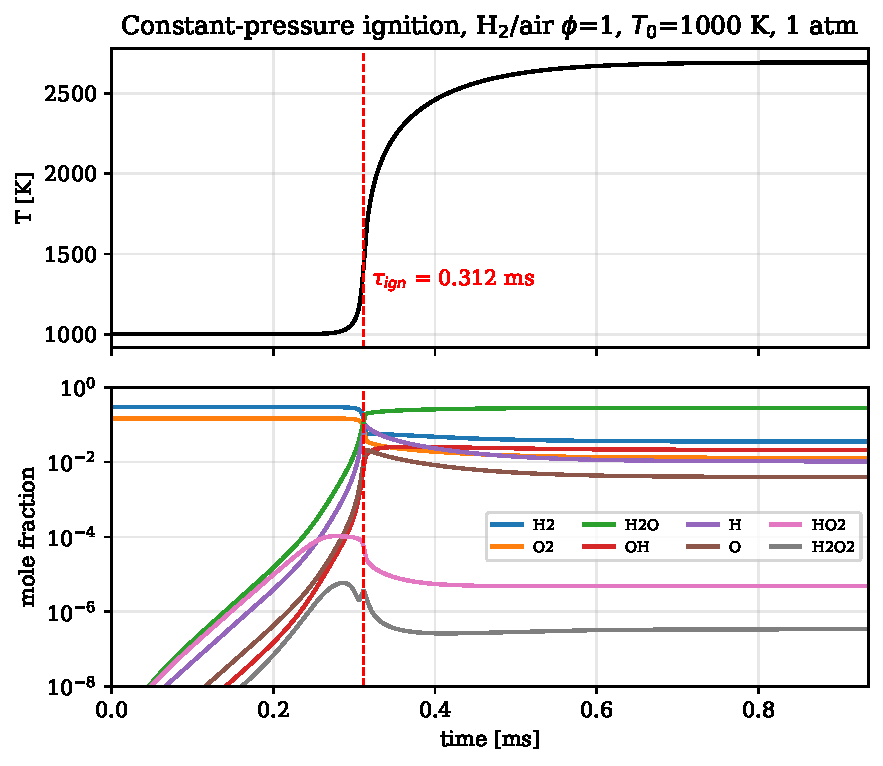
\includegraphics[width=0.85\textwidth]{ignition_0D}
\caption{Constant-pressure ignition of stoichiometric \ce{H_2}/air at $T_0=\SI{1000}{\kelvin}$,
1 atm (\code{h2o2.yaml}). Top: temperature. Bottom: species on a log scale. The ignition delay
$\tau_{ign}$ is the time of maximum $\dd T/\dd t$.}
\label{fig:ign}
\end{figure}

Three phases are visible:
\begin{enumerate}
  \item \textbf{Induction.} $T$ is flat, but radicals (H, O, OH) grow \emph{exponentially}: straight
        lines on the log plot, as predicted by the branching analysis of \secref{sec:h2chain}. Very
        little heat is released because the radical concentrations are still tiny.
  \item \textbf{Ignition.} Once radicals reach $\sim10^{-3}$, fuel consumption and recombination
        (heat release) become significant. Higher $T$ accelerates branching even more. This
        feedback makes $T$ jump by $\sim\SI{1500}{\kelvin}$ in microseconds.
  \item \textbf{Equilibration.} Radicals recombine slowly (three-body reactions) and $T$ creeps
        towards $\Tad$, the same value \code{equilibrate("HP")} gives.
\end{enumerate}

\begin{figure}[H]
\centering
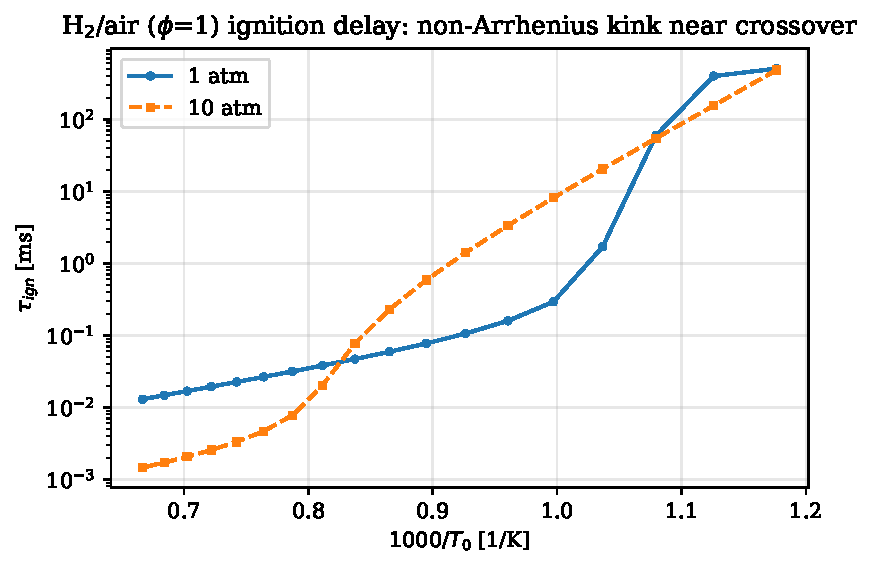
\includegraphics[width=0.85\textwidth]{ignition_delay}
\caption{Ignition delay vs.\ $1000/T_0$. At high $T$ the curves are nearly straight (Arrhenius).
Near the crossover temperature (\figref{fig:arrh}) the slope changes sharply: below it, R5 steals H
atoms and ignition must proceed through slower \ce{HO_2}/\ce{H_2O_2} chemistry. At 10~atm the
crossover moves to higher $T$, which is why at intermediate temperatures high pressure ignites
\emph{later}.}
\label{fig:taudelay}
\end{figure}

\section{Damköhler number and frozen chemistry}

Compare a flow time $\tau_{\rm flow}$ (residence time in a combustor, time for strain to remove
heat in a flame) with a chemical time $\tau_{\rm chem}$ (e.g.\ $\tau_{ign}$):
\begin{equation}
  \mathrm{Da}=\frac{\tau_{\rm flow}}{\tau_{\rm chem}} .
\end{equation}
\begin{itemize}
  \item $\mathrm{Da}\gg1$: chemistry finishes; the state is close to equilibrium.
  \item $\mathrm{Da}\ll1$: chemistry has no time; composition is \emph{frozen}. This is how CO and
        unburnt hydrocarbons escape from engines.
  \item $\mathrm{Da}\sim1$: chemistry and flow compete, as in extinction, ignition and pollutant
        formation.
\end{itemize}
The Damköhler number will reappear as the parameter of the S-curve in non-premixed flames
(\secref{sec:scurve}).

\section{In Cantera}

\begin{lstlisting}
import cantera as ct, numpy as np
gas = ct.Solution("h2o2.yaml")
gas.set_equivalence_ratio(1.0, "H2", "O2:1, N2:3.76")
gas.TP = 1000.0, ct.one_atm

reactor = ct.IdealGasConstPressureReactor(gas, clone=True)  # clone: own copy of gas
net = ct.ReactorNet([reactor])
states = ct.SolutionArray(gas, extra=["t"])
while net.time < 2e-3:
    net.step()                                   # adaptive implicit step (CVODES)
    states.append(reactor.phase.state, t=net.time)

tau = states.t[np.argmax(np.gradient(states.T, states.t))]
\end{lstlisting}

\begin{warning}[Cantera 3.2 API changes]
\code{reactor.thermo} is deprecated in favour of \code{reactor.phase}. The \code{clone} argument
will default to \code{True} after 3.2. Pass it explicitly to avoid warnings and surprises: with
\code{clone=False} the reactor and your \code{gas} object share one state, so reading
\code{gas.T} during integration gives the reactor temperature.
\end{warning}

\begin{selfcheck}
\begin{enumerate}
  \item Why does the 0D reactor's final temperature equal \code{equilibrate("HP")} exactly?
        (Hint: \secref{sec:reverse}.)
  \item In \figref{fig:ign}, which species peaks \emph{before} ignition, and why?
        (Hint: R5 at \SI{1000}{\kelvin}.)
  \item What is the Damköhler number of a gas turbine combustor with residence time
        \SI{5}{\milli\second} burning a mixture whose $\tau_{ign}$ is \SI{0.1}{\milli\second}?
\end{enumerate}
\end{selfcheck}
